% Options for packages loaded elsewhere
\PassOptionsToPackage{unicode}{hyperref}
\PassOptionsToPackage{hyphens}{url}
\PassOptionsToPackage{dvipsnames,svgnames,x11names}{xcolor}
%
\documentclass[
  11pt,
]{article}

\usepackage{amsmath,amssymb}
\usepackage{iftex}
\ifPDFTeX
  \usepackage[T1]{fontenc}
  \usepackage[utf8]{inputenc}
  \usepackage{textcomp} % provide euro and other symbols
\else % if luatex or xetex
  \usepackage{unicode-math}
  \defaultfontfeatures{Scale=MatchLowercase}
  \defaultfontfeatures[\rmfamily]{Ligatures=TeX,Scale=1}
\fi
\usepackage{lmodern}
\ifPDFTeX\else  
    % xetex/luatex font selection
\fi
% Use upquote if available, for straight quotes in verbatim environments
\IfFileExists{upquote.sty}{\usepackage{upquote}}{}
\IfFileExists{microtype.sty}{% use microtype if available
  \usepackage[]{microtype}
  \UseMicrotypeSet[protrusion]{basicmath} % disable protrusion for tt fonts
}{}
\makeatletter
\@ifundefined{KOMAClassName}{% if non-KOMA class
  \IfFileExists{parskip.sty}{%
    \usepackage{parskip}
  }{% else
    \setlength{\parindent}{0pt}
    \setlength{\parskip}{6pt plus 2pt minus 1pt}}
}{% if KOMA class
  \KOMAoptions{parskip=half}}
\makeatother
\usepackage{xcolor}
\usepackage[margin=0.75in]{geometry}
\setlength{\emergencystretch}{3em} % prevent overfull lines
\setcounter{secnumdepth}{-\maxdimen} % remove section numbering
% Make \paragraph and \subparagraph free-standing
\ifx\paragraph\undefined\else
  \let\oldparagraph\paragraph
  \renewcommand{\paragraph}[1]{\oldparagraph{#1}\mbox{}}
\fi
\ifx\subparagraph\undefined\else
  \let\oldsubparagraph\subparagraph
  \renewcommand{\subparagraph}[1]{\oldsubparagraph{#1}\mbox{}}
\fi

\usepackage{color}
\usepackage{fancyvrb}
\newcommand{\VerbBar}{|}
\newcommand{\VERB}{\Verb[commandchars=\\\{\}]}
\DefineVerbatimEnvironment{Highlighting}{Verbatim}{commandchars=\\\{\}}
% Add ',fontsize=\small' for more characters per line
\usepackage{framed}
\definecolor{shadecolor}{RGB}{241,243,245}
\newenvironment{Shaded}{\begin{snugshade}}{\end{snugshade}}
\newcommand{\AlertTok}[1]{\textcolor[rgb]{0.68,0.00,0.00}{#1}}
\newcommand{\AnnotationTok}[1]{\textcolor[rgb]{0.37,0.37,0.37}{#1}}
\newcommand{\AttributeTok}[1]{\textcolor[rgb]{0.40,0.45,0.13}{#1}}
\newcommand{\BaseNTok}[1]{\textcolor[rgb]{0.68,0.00,0.00}{#1}}
\newcommand{\BuiltInTok}[1]{\textcolor[rgb]{0.00,0.23,0.31}{#1}}
\newcommand{\CharTok}[1]{\textcolor[rgb]{0.13,0.47,0.30}{#1}}
\newcommand{\CommentTok}[1]{\textcolor[rgb]{0.37,0.37,0.37}{#1}}
\newcommand{\CommentVarTok}[1]{\textcolor[rgb]{0.37,0.37,0.37}{\textit{#1}}}
\newcommand{\ConstantTok}[1]{\textcolor[rgb]{0.56,0.35,0.01}{#1}}
\newcommand{\ControlFlowTok}[1]{\textcolor[rgb]{0.00,0.23,0.31}{#1}}
\newcommand{\DataTypeTok}[1]{\textcolor[rgb]{0.68,0.00,0.00}{#1}}
\newcommand{\DecValTok}[1]{\textcolor[rgb]{0.68,0.00,0.00}{#1}}
\newcommand{\DocumentationTok}[1]{\textcolor[rgb]{0.37,0.37,0.37}{\textit{#1}}}
\newcommand{\ErrorTok}[1]{\textcolor[rgb]{0.68,0.00,0.00}{#1}}
\newcommand{\ExtensionTok}[1]{\textcolor[rgb]{0.00,0.23,0.31}{#1}}
\newcommand{\FloatTok}[1]{\textcolor[rgb]{0.68,0.00,0.00}{#1}}
\newcommand{\FunctionTok}[1]{\textcolor[rgb]{0.28,0.35,0.67}{#1}}
\newcommand{\ImportTok}[1]{\textcolor[rgb]{0.00,0.46,0.62}{#1}}
\newcommand{\InformationTok}[1]{\textcolor[rgb]{0.37,0.37,0.37}{#1}}
\newcommand{\KeywordTok}[1]{\textcolor[rgb]{0.00,0.23,0.31}{#1}}
\newcommand{\NormalTok}[1]{\textcolor[rgb]{0.00,0.23,0.31}{#1}}
\newcommand{\OperatorTok}[1]{\textcolor[rgb]{0.37,0.37,0.37}{#1}}
\newcommand{\OtherTok}[1]{\textcolor[rgb]{0.00,0.23,0.31}{#1}}
\newcommand{\PreprocessorTok}[1]{\textcolor[rgb]{0.68,0.00,0.00}{#1}}
\newcommand{\RegionMarkerTok}[1]{\textcolor[rgb]{0.00,0.23,0.31}{#1}}
\newcommand{\SpecialCharTok}[1]{\textcolor[rgb]{0.37,0.37,0.37}{#1}}
\newcommand{\SpecialStringTok}[1]{\textcolor[rgb]{0.13,0.47,0.30}{#1}}
\newcommand{\StringTok}[1]{\textcolor[rgb]{0.13,0.47,0.30}{#1}}
\newcommand{\VariableTok}[1]{\textcolor[rgb]{0.07,0.07,0.07}{#1}}
\newcommand{\VerbatimStringTok}[1]{\textcolor[rgb]{0.13,0.47,0.30}{#1}}
\newcommand{\WarningTok}[1]{\textcolor[rgb]{0.37,0.37,0.37}{\textit{#1}}}

\providecommand{\tightlist}{%
  \setlength{\itemsep}{0pt}\setlength{\parskip}{0pt}}\usepackage{longtable,booktabs,array}
\usepackage{calc} % for calculating minipage widths
% Correct order of tables after \paragraph or \subparagraph
\usepackage{etoolbox}
\makeatletter
\patchcmd\longtable{\par}{\if@noskipsec\mbox{}\fi\par}{}{}
\makeatother
% Allow footnotes in longtable head/foot
\IfFileExists{footnotehyper.sty}{\usepackage{footnotehyper}}{\usepackage{footnote}}
\makesavenoteenv{longtable}
\usepackage{graphicx}
\makeatletter
\def\maxwidth{\ifdim\Gin@nat@width>\linewidth\linewidth\else\Gin@nat@width\fi}
\def\maxheight{\ifdim\Gin@nat@height>\textheight\textheight\else\Gin@nat@height\fi}
\makeatother
% Scale images if necessary, so that they will not overflow the page
% margins by default, and it is still possible to overwrite the defaults
% using explicit options in \includegraphics[width, height, ...]{}
\setkeys{Gin}{width=\maxwidth,height=\maxheight,keepaspectratio}
% Set default figure placement to htbp
\makeatletter
\def\fps@figure{htbp}
\makeatother

\usepackage{fvextra}
\DefineVerbatimEnvironment{Highlighting}{Verbatim}{breaklines,commandchars=\\\{\}}
\DefineVerbatimEnvironment{OutputCode}{Verbatim}{breaklines,commandchars=\\\{\}}
\fvset{breaksymbolleft={}, breakindent=1em}
\makeatletter
\@ifpackageloaded{caption}{}{\usepackage{caption}}
\AtBeginDocument{%
\ifdefined\contentsname
  \renewcommand*\contentsname{Table of contents}
\else
  \newcommand\contentsname{Table of contents}
\fi
\ifdefined\listfigurename
  \renewcommand*\listfigurename{List of Figures}
\else
  \newcommand\listfigurename{List of Figures}
\fi
\ifdefined\listtablename
  \renewcommand*\listtablename{List of Tables}
\else
  \newcommand\listtablename{List of Tables}
\fi
\ifdefined\figurename
  \renewcommand*\figurename{Figure}
\else
  \newcommand\figurename{Figure}
\fi
\ifdefined\tablename
  \renewcommand*\tablename{Table}
\else
  \newcommand\tablename{Table}
\fi
}
\@ifpackageloaded{float}{}{\usepackage{float}}
\floatstyle{ruled}
\@ifundefined{c@chapter}{\newfloat{codelisting}{h}{lop}}{\newfloat{codelisting}{h}{lop}[chapter]}
\floatname{codelisting}{Listing}
\newcommand*\listoflistings{\listof{codelisting}{List of Listings}}
\makeatother
\makeatletter
\makeatother
\makeatletter
\@ifpackageloaded{caption}{}{\usepackage{caption}}
\@ifpackageloaded{subcaption}{}{\usepackage{subcaption}}
\makeatother
\ifLuaTeX
  \usepackage{selnolig}  % disable illegal ligatures
\fi
\usepackage{bookmark}

\IfFileExists{xurl.sty}{\usepackage{xurl}}{} % add URL line breaks if available
\urlstyle{same} % disable monospaced font for URLs
\hypersetup{
  pdftitle={Assignment 1},
  pdfauthor={Nick Climaco},
  colorlinks=true,
  linkcolor={blue},
  filecolor={Maroon},
  citecolor={Blue},
  urlcolor={Blue},
  pdfcreator={LaTeX via pandoc}}

\title{Assignment 1}
\author{Nick Climaco}
\date{September 3, 2024}

\begin{document}
\maketitle

\renewcommand*\contentsname{Table of contents}
{
\hypersetup{linkcolor=}
\setcounter{tocdepth}{3}
\tableofcontents
}
\newpage

\section{01- Assignment}\label{assignment}

\subsubsection{1) Successfully downloaded Simio and
Python}\label{successfully-downloaded-simio-and-python}

I have downloaded Simio and Python

\begin{figure}[H]

{\centering 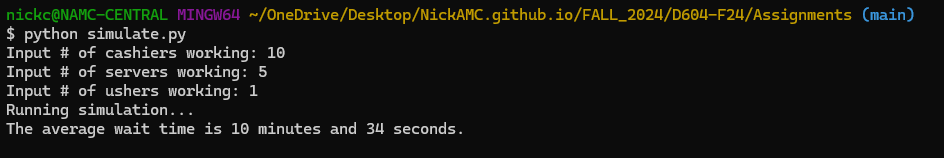
\includegraphics{01-assignment_files/figure-pdf/cell-3-2-image.png}

}

\caption{image.png}

\end{figure}%%
\begin{figure}[H]

{\centering 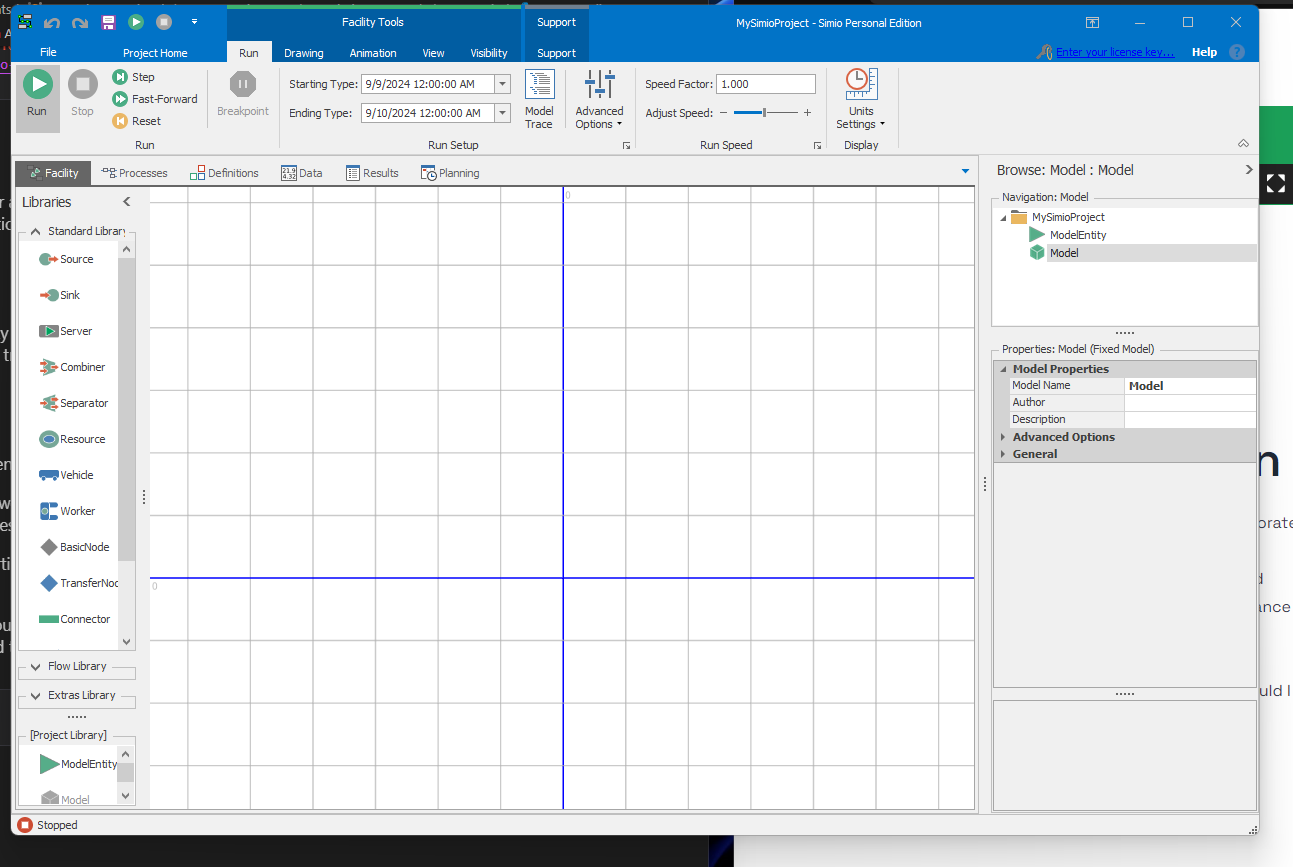
\includegraphics{01-assignment_files/figure-pdf/cell-3-1-image-2.png}

}

\caption{image-2.png}

\end{figure}%

\subsubsection{2) Guided Tutorial on
Simpy}\label{guided-tutorial-on-simpy}

https://realpython.com/simpy-simulating-with-python/\#what-simulation-is

\begin{Shaded}
\begin{Highlighting}[]
\ImportTok{import}\NormalTok{ random}
\ImportTok{import}\NormalTok{ statistics}

\ImportTok{import}\NormalTok{ simpy}

\NormalTok{wait\_times }\OperatorTok{=}\NormalTok{ []}


\KeywordTok{class}\NormalTok{ Theater(}\BuiltInTok{object}\NormalTok{):}
    \KeywordTok{def} \FunctionTok{\_\_init\_\_}\NormalTok{(}\VariableTok{self}\NormalTok{, env, num\_cashiers, num\_servers, num\_ushers):}
        \VariableTok{self}\NormalTok{.env }\OperatorTok{=}\NormalTok{ env}
        \VariableTok{self}\NormalTok{.cashier }\OperatorTok{=}\NormalTok{ simpy.Resource(env, num\_cashiers)}
        \VariableTok{self}\NormalTok{.server }\OperatorTok{=}\NormalTok{ simpy.Resource(env, num\_servers)}
        \VariableTok{self}\NormalTok{.usher }\OperatorTok{=}\NormalTok{ simpy.Resource(env, num\_ushers)}

    \KeywordTok{def}\NormalTok{ purchase\_ticket(}\VariableTok{self}\NormalTok{, moviegoer):}
        \ControlFlowTok{yield} \VariableTok{self}\NormalTok{.env.timeout(random.randint(}\DecValTok{1}\NormalTok{, }\DecValTok{3}\NormalTok{))}

    \KeywordTok{def}\NormalTok{ check\_ticket(}\VariableTok{self}\NormalTok{, moviegoer):}
        \ControlFlowTok{yield} \VariableTok{self}\NormalTok{.env.timeout(}\DecValTok{3} \OperatorTok{/} \DecValTok{60}\NormalTok{)}

    \KeywordTok{def}\NormalTok{ sell\_food(}\VariableTok{self}\NormalTok{, moviegoer):}
        \ControlFlowTok{yield} \VariableTok{self}\NormalTok{.env.timeout(random.randint(}\DecValTok{1}\NormalTok{, }\DecValTok{5}\NormalTok{))}


\KeywordTok{def}\NormalTok{ go\_to\_movies(env, moviegoer, theater):}
    \CommentTok{\# Moviegoer arrives at the theater}
\NormalTok{    arrival\_time }\OperatorTok{=}\NormalTok{ env.now}

    \ControlFlowTok{with}\NormalTok{ theater.cashier.request() }\ImportTok{as}\NormalTok{ request:}
        \ControlFlowTok{yield}\NormalTok{ request}
        \ControlFlowTok{yield}\NormalTok{ env.process(theater.purchase\_ticket(moviegoer))}

    \ControlFlowTok{with}\NormalTok{ theater.usher.request() }\ImportTok{as}\NormalTok{ request:}
        \ControlFlowTok{yield}\NormalTok{ request}
        \ControlFlowTok{yield}\NormalTok{ env.process(theater.check\_ticket(moviegoer))}

    \ControlFlowTok{if}\NormalTok{ random.choice([}\VariableTok{True}\NormalTok{, }\VariableTok{False}\NormalTok{]):}
        \ControlFlowTok{with}\NormalTok{ theater.server.request() }\ImportTok{as}\NormalTok{ request:}
            \ControlFlowTok{yield}\NormalTok{ request}
            \ControlFlowTok{yield}\NormalTok{ env.process(theater.sell\_food(moviegoer))}

    \CommentTok{\# Moviegoer heads into the theater}
\NormalTok{    wait\_times.append(env.now }\OperatorTok{{-}}\NormalTok{ arrival\_time)}


\KeywordTok{def}\NormalTok{ run\_theater(env, num\_cashiers, num\_servers, num\_ushers):}
\NormalTok{    theater }\OperatorTok{=}\NormalTok{ Theater(env, num\_cashiers, num\_servers, num\_ushers)}

    \ControlFlowTok{for}\NormalTok{ moviegoer }\KeywordTok{in} \BuiltInTok{range}\NormalTok{(}\DecValTok{3}\NormalTok{):}
\NormalTok{        env.process(go\_to\_movies(env, moviegoer, theater))}

    \ControlFlowTok{while} \VariableTok{True}\NormalTok{:}
        \ControlFlowTok{yield}\NormalTok{ env.timeout(}\FloatTok{0.20}\NormalTok{)  }\CommentTok{\# Wait a bit before generating a new person}

\NormalTok{        moviegoer }\OperatorTok{+=} \DecValTok{1}
\NormalTok{        env.process(go\_to\_movies(env, moviegoer, theater))}


\KeywordTok{def}\NormalTok{ get\_average\_wait\_time(wait\_times):}
\NormalTok{    average\_wait }\OperatorTok{=}\NormalTok{ statistics.mean(wait\_times)}
    \CommentTok{\# Pretty print the results}
\NormalTok{    minutes, frac\_minutes }\OperatorTok{=} \BuiltInTok{divmod}\NormalTok{(average\_wait, }\DecValTok{1}\NormalTok{)}
\NormalTok{    seconds }\OperatorTok{=}\NormalTok{ frac\_minutes }\OperatorTok{*} \DecValTok{60}
    \ControlFlowTok{return} \BuiltInTok{round}\NormalTok{(minutes), }\BuiltInTok{round}\NormalTok{(seconds)}


\KeywordTok{def}\NormalTok{ get\_user\_input():}
\NormalTok{    num\_cashiers }\OperatorTok{=} \BuiltInTok{input}\NormalTok{(}\StringTok{"Input \# of cashiers working: "}\NormalTok{)}
\NormalTok{    num\_servers }\OperatorTok{=} \BuiltInTok{input}\NormalTok{(}\StringTok{"Input \# of servers working: "}\NormalTok{)}
\NormalTok{    num\_ushers }\OperatorTok{=} \BuiltInTok{input}\NormalTok{(}\StringTok{"Input \# of ushers working: "}\NormalTok{)}
\NormalTok{    params }\OperatorTok{=}\NormalTok{ [num\_cashiers, num\_servers, num\_ushers]}
    \ControlFlowTok{if} \BuiltInTok{all}\NormalTok{(}\BuiltInTok{str}\NormalTok{(i).isdigit() }\ControlFlowTok{for}\NormalTok{ i }\KeywordTok{in}\NormalTok{ params):  }\CommentTok{\# Check input is valid}
\NormalTok{        params }\OperatorTok{=}\NormalTok{ [}\BuiltInTok{int}\NormalTok{(x) }\ControlFlowTok{for}\NormalTok{ x }\KeywordTok{in}\NormalTok{ params]}
    \ControlFlowTok{else}\NormalTok{:}
        \BuiltInTok{print}\NormalTok{(}
            \StringTok{"Could not parse input. Simulation will use default values:"}\NormalTok{,}
            \StringTok{"}\CharTok{\textbackslash{}n}\StringTok{1 cashier, 1 server, 1 usher."}\NormalTok{,}
\NormalTok{        )}
\NormalTok{        params }\OperatorTok{=}\NormalTok{ [}\DecValTok{1}\NormalTok{, }\DecValTok{1}\NormalTok{, }\DecValTok{1}\NormalTok{]}
    \ControlFlowTok{return}\NormalTok{ params}


\KeywordTok{def}\NormalTok{ main():}
    \CommentTok{\# Setup}
\NormalTok{    random.seed(}\DecValTok{42}\NormalTok{)}
\NormalTok{    num\_cashiers, num\_servers, num\_ushers }\OperatorTok{=}\NormalTok{ get\_user\_input()}

    \CommentTok{\# Run the simulation}
\NormalTok{    env }\OperatorTok{=}\NormalTok{ simpy.Environment()}
\NormalTok{    env.process(run\_theater(env, num\_cashiers, num\_servers, num\_ushers))}
\NormalTok{    env.run(until}\OperatorTok{=}\DecValTok{90}\NormalTok{)}

    \CommentTok{\# View the results}
\NormalTok{    mins, secs }\OperatorTok{=}\NormalTok{ get\_average\_wait\_time(wait\_times)}
    \BuiltInTok{print}\NormalTok{(}
        \StringTok{"Running simulation..."}\NormalTok{,}
        \SpecialStringTok{f"}\CharTok{\textbackslash{}n}\SpecialStringTok{The average wait time is }\SpecialCharTok{\{}\NormalTok{mins}\SpecialCharTok{\}}\SpecialStringTok{ minutes and }\SpecialCharTok{\{}\NormalTok{secs}\SpecialCharTok{\}}\SpecialStringTok{ seconds."}\NormalTok{,}
\NormalTok{    )}


\ControlFlowTok{if} \VariableTok{\_\_name\_\_} \OperatorTok{==} \StringTok{"\_\_main\_\_"}\NormalTok{:}
\NormalTok{    main()}
\end{Highlighting}
\end{Shaded}

\begin{verbatim}
Running simulation... 
The average wait time is 4 minutes and 12 seconds.
\end{verbatim}

Inputs:10 cashiers, 10 servers and 2 usher

\subsubsection{3) Simio Case Study}\label{simio-case-study}

\href{https://www.simio.com/projects/deciding-where-to-build-a-new-distribution-center/}{Deciding
Where To Build A New Distribution Center}

\paragraph{Problem:}\label{problem}

A company is looking for a new location to build an additional
distribution center. They want to assess the most cost effective
location in relation to the existing distribution center.

\paragraph{Solution:}\label{solution}

Students at the University of Pittsburgh used Simio to simulate the
truck route, while considering these factors: weekly replenishment
schedule, travel time, mileage, and pre-selected truck routes.

\paragraph{Result:}\label{result}

If the new distribution center is built in Akron, OH:

\begin{itemize}
\item
  12\% of the yearly hours worked would be overtime
\item
  1,234,199 yearly vehicle miles
\item
  A yearly logistic cost of \$1,703,195
\end{itemize}

To build in Grove City, OH results in:

\begin{itemize}
\item
  18\% of the hours in overtime
\item
  1,491,493 yearly vehicle miles
\item
  \$2,085,260 in yearly operating costs
\end{itemize}

Building in Sharonville, OH would result in:

\begin{itemize}
\item
  29\% of the total work hours being overtime hours
\item
  1,754,339 yearly vehicle miles
\item
  \$2,420,988 yearly operating costs
\end{itemize}

The simulation demonstrated that Akron will be the best location to
build.

\paragraph{Short essay}\label{short-essay}

Other factors to build a stronger and more accurate model is to consider
the local work force availability. The company must survey the whether
or not the local population already possesses the skills required to
operate a distribution center. If the local workforce lacks the skills
then the company must bring in workers from other regions to operate and
possibly train the local workers which would increase the operating
costs. Conversely, if the local workforce already possesses the required
skills then the company will not have to bring workers from other
regions and this would lower operating costs for the distribution
center. The company could quantify this data with the local population's
average age and of those local worker how many of them has a high school
degree, undergraduate degree, or trade school degree. Implementing this
component in the simulation can display a more comprehensive
understanding of the potential location.

Another factor to consider in this simulation model is the current
infrastructure in the area. The model can simulate whether the company
has to build a distribution center from the ground or if there exists
infrastructure such as empty warehouses or distribution centers from
defunct companies. Using these building would greater reduce the cost
and time to set up a new distribution center. The infrastructure data of
the region could be passed into the model where it would assess the most
cost effective and optimal location to place a distribution center.

With these additional factors, data on local workforce and current
infrastructure, the model becomes more comprehensive and possibly offer
a more accurate projection of the costs and logistics of setting up a
new distribution center. Ultimately, this model would supply important
information to the company's decision makers e.g.~the executives.



\end{document}
